\documentclass[12pt]{article}

\usepackage{amsmath, mathtools}
\usepackage{amsfonts}
\usepackage{amssymb}
\usepackage{graphicx}
\usepackage{colortbl}
\usepackage{xr}
\usepackage{hyperref}
\usepackage{longtable}
\usepackage{xfrac}
\usepackage{tabularx}
\usepackage{float}
\usepackage{siunitx}
\usepackage{booktabs}
\usepackage{caption}
\usepackage{pdflscape}
\usepackage{afterpage}   
\usepackage{graphicx}

\usepackage[round]{natbib}

%\usepackage{refcheck}

\hypersetup{
	bookmarks=true,         % show bookmarks bar?
	colorlinks=true,       % false: boxed links; true: colored links
	linkcolor=red,          % color of internal links (change box color with
	%linkbordercolor)
	citecolor=green,        % color of links to bibliography
	filecolor=magenta,      % color of file links
	urlcolor=cyan           % color of external links
}

%% Comments

\usepackage{color}

\newif\ifcomments\commentstrue %displays comments
%\newif\ifcomments\commentsfalse %so that comments do not display

\ifcomments
\newcommand{\authornote}[3]{\textcolor{#1}{[#3 ---#2]}}
\newcommand{\todo}[1]{\textcolor{red}{[TODO: #1]}}
\else
\newcommand{\authornote}[3]{}
\newcommand{\todo}[1]{}
\fi

\newcommand{\wss}[1]{\authornote{blue}{SS}{#1}} 
\newcommand{\plt}[1]{\authornote{magenta}{TPLT}{#1}} %For explanation of the template
\newcommand{\an}[1]{\authornote{cyan}{Author}{#1}}


\newcommand{\progname}{Software Eng 4G06} % PUT YOUR PROGRAM NAME HERE
\newcommand{\authname}{Team 2, Parnas' Pals
	\\ Jared Bentvelsen
	\\ Bassel Rezkalla
	\\ Yuvraj Randhawa
	\\ Dimitri Tsampiras
	\\ Matthew McCracken} % AUTHOR NAMES                  

\usepackage{hyperref}
\hypersetup{colorlinks=true, linkcolor=blue, citecolor=blue, filecolor=blue,
	urlcolor=blue, unicode=false}
\urlstyle{same}



% For easy change of table widths
\newcommand{\colZwidth}{1.0\textwidth}
\newcommand{\colAwidth}{0.13\textwidth}
\newcommand{\colBwidth}{0.82\textwidth}
\newcommand{\colCwidth}{0.1\textwidth}
\newcommand{\colDwidth}{0.05\textwidth}
\newcommand{\colEwidth}{0.8\textwidth}
\newcommand{\colFwidth}{0.17\textwidth}
\newcommand{\colGwidth}{0.5\textwidth}
\newcommand{\colHwidth}{0.28\textwidth}

% Used so that cross-references have a meaningful prefix
\newcounter{defnum} %Definition Number
\newcommand{\dthedefnum}{GD\thedefnum}
\newcommand{\dref}[1]{GD\ref{#1}}
\newcounter{datadefnum} %Datadefinition Number
\newcommand{\ddthedatadefnum}{DD\thedatadefnum}
\newcommand{\ddref}[1]{DD\ref{#1}}
\newcounter{theorynum} %Theory Number
\newcommand{\tthetheorynum}{T\thetheorynum}
\newcommand{\tref}[1]{T\ref{#1}}
\newcounter{tablenum} %Table Number
\newcommand{\tbthetablenum}{T\thetablenum}
\newcommand{\tbref}[1]{TB\ref{#1}}
\newcounter{assumpnum} %Assumption Number
\newcommand{\atheassumpnum}{P\theassumpnum}
\newcommand{\aref}[1]{A\ref{#1}}
\newcounter{goalnum} %Goal Number
\newcommand{\gthegoalnum}{P\thegoalnum}
\newcommand{\gsref}[1]{GS\ref{#1}}
\newcounter{instnum} %Instance Number
\newcommand{\itheinstnum}{IM\theinstnum}
\newcommand{\iref}[1]{IM\ref{#1}}
\newcounter{reqnum} %Requirement Number
\newcommand{\rthereqnum}{P\thereqnum}
\newcommand{\rref}[1]{R\ref{#1}}
\newcounter{nfrnum} %NFR Number
\newcommand{\rthenfrnum}{NFR\thenfrnum}
\newcommand{\nfrref}[1]{NFR\ref{#1}}
\newcounter{lcnum} %Likely change number
\newcommand{\lthelcnum}{LC\thelcnum}
\newcommand{\lcref}[1]{LC\ref{#1}}

\usepackage{fullpage}

\newcommand{\deftheory}[9][Not Applicable]
{
	\newpage
	\noindent \rule{\textwidth}{0.5mm}
	
	\paragraph{RefName: } \textbf{#2} \phantomsection 
	\label{#2}
	
	\paragraph{Label:} #3
	
	\noindent \rule{\textwidth}{0.5mm}
	
	\paragraph{Equation:}
	
	#4
	
	\paragraph{Description:}
	
	#5
	
	\paragraph{Notes:}
	
	#6
	
	\paragraph{Source:}
	
	#7
	
	\paragraph{Ref.\ By:}
	
	#8
	
	\paragraph{Preconditions for \hyperref[#2]{#2}:}
	\label{#2_precond}
	
	#9
	
	\paragraph{Derivation for \hyperref[#2]{#2}:}
	\label{#2_deriv}
	
	#1
	
	\noindent \rule{\textwidth}{0.5mm}
	
}

\begin{document}

\title{Software Requirements Specification for \progname: subtitle describing software} 
\author{\authname}
\date{\today}
	
\maketitle

~\newpage

\pagenumbering{roman}

\tableofcontents

~\newpage

\section*{Revision History}

\begin{tabularx}{\textwidth}{p{3cm}p{2cm}X}
\toprule {\bf Date} & {\bf Version} & {\bf Notes}\\
\midrule
Date 1 & 1.0 & Notes\\
Date 2 & 1.1 & Notes\\
\bottomrule
\end{tabularx}

~\newpage


\section{The Purpose of the Project}
\subsection{The User Business or Background of the Project Effort}
\subsection{Goals of the Project}


\section{Project Drivers}
\subsection{The Purpose of the Project}
  \subsubsection{The User Business or Background of the Project Effort}
  \noindent
  With the increase in media consumption across the world, there has been a greater focus on several previously underrepresented or inaccessable niches, such as health and fitness. Despite the growth and presence of fitness in social media, there are still large barriers to entry that make it intimidating to get started or get accurate information that would aid individuals in their fitness journeys. A lot of the media available online is either behind a paywall, or structured in undigestible video and written formats. The lack of a free, centralized system that contains media generated and verified by fitness enthusiasts alike spurred the idea for this application. This application aims to bridge the gap that exists in the online fitness world by allowing individuals to create and track workouts of their own, search and share workouts created by others, and review and discuss what they find personally works and doesn't work for them. Creating a collaborative online fitness environment allows individuals to start or expand their fitness journey without looking in numerous locations or paying money for programs that may not work for them. 
\subsection{Stakeholders}
\begin{enumerate}
	\item Fitness Enthusiasts - Anyone interested in exploring other fitness routines, creating their own routines, and tracking their own personal progression towards goals.
	\item Personal Trainers - Olympian provides the ideal platform for trainers to share routines and goals with their clients.
	\item Fitness Advertisers - One avenue of monetization that Olympian could take is running advertisements. Although these advertisements could fall into any category, the largest stakeholders will be Fitness Advertisers,
	as the users of Olympian will be heavily involved with fitness, and thus most likely to buy fitness products.
\end{enumerate} 

\section{Project Constraints}
\subsection{Mandated Constraints} 
\subsubsection{Solution Constraints}
\begin{enumerate}
	\item
	\textbf{Description: } The product shall operate its back-end server with Node.js. \\
	\textbf{Rationale: } The product depends on the functionality provided by many libraries unique to Node.js. \\
	\textbf{Fit Criterion: } All back-end server libraries used are Node.js libraries, with a Node.js back-end. \\
\end{enumerate}
\subsubsection{Implementation Environment of the Current System}
The product will be launched as a web-app on the internet, and as a mobile app. There is no hardware or otherwise physical integration of the product.
\subsubsection{Partner or Collaborative Applications}
N/A
\subsubsection{Off-the-Shelf Software}
N/A
\subsubsection{Anticipated Workplace Environment}
N/A
\subsubsection{Schedule Constraints}
The product timeline will follow the schedule as laid out in the course outline by Dr. Smith. \\
\newline
\begin{tabular}{ p{9.7cm} l r}
	
	Team Formed, Project Selected & September 19 & 0\% \\
	
	Problem Statement, Development Plan & September 26 &
	2\% \\
	
	Requirements Document Revision 0 & October 5 & 5$\%^{\dagger, \ddagger}$ \\
	
	Hazard Analysis 0 & October 19 & 3$\%^\dagger$ \\
	
	V\&V Plan Revision 0 & November 2 & 5$\%^{\dagger, \ddagger}$ \\
	
	Proof of Concept Demonstration & November 14--25 & 5$\%^*$ \\
	
	Design Document Revision 0 & January 18 & 5$\%^{\dagger, \ddagger}$ \\
	
	Revision 0 Demonstration & February 6--February 17 & 10$\%^*$\\
	
	V\&V Report Revision 0 & March 8 & 5$\%^{\dagger, \ddagger}$ \\
	
	Final Demonstration (Revision 1) & March 20--March 31 &  20$\%^*$ \\
	
	EXPO Demonstration & April TBD & 10$\%^*$ \\
	
	Final Documentation (Revision 1)\newline 
	- Problem Statement\newline
	- Development Plan\newline
	- Requirements Document\newline
	- Hazard Analysis\newline
	- Design Document\newline
	- V\&V Plan\newline
	- V\&V Report\newline
	- User's Guide\newline
	- Source Code\newline &  April 5 & 30$\%^{*, \ddagger}$\\
	
\end{tabular}
\subsubsection{Budget Constraints}
N/A
\subsubsection{Enterprise Constraints}
N/A

\subsection{Naming Conventions and Terminology}
Below is a glossary of terms, acronyms and abbreviations used by stakeholders involved in the product's scope:
\begin{itemize}
	\item \textbf{Repetitions: } The number of times a motion will be repeated.
	\item \textbf{Exercise: } An entity describing a physical movement to be performed with optional descriptors and any combination of the following quantifiers: Repetitions, Sets, Weight, Distance, Time, and Rest Time. 
	\item \textbf{Routine: } A routine (or workout routine) is composed of a sequence of exercises performed in order.
\end{itemize}
\subsection{Relevant Facts and Assumptions}
N/A
\section{Functional Requirements}
\subsection{The Scope of the Work}
\subsection{Business Data Model and Data Directory}
\subsection{The Scope of the Product}
\subsection{Functional Requirements}
\noindent \begin{itemize}

\item[R\refstepcounter{reqnum}\thereqnum \label{R_Inputs}:]
Description: The system shall allow the user to create a workout routine.
\\ Rationale: To allow the user to save their own workout routines.
\\ Fit Criterion: The user created routines are accessible after creation.

\item[R\refstepcounter{reqnum}\thereqnum \label{R_Inputs}:]
Description: The system shall allow the user to add and remove individual exercises in order to a created workout routine, with a maximum of 20 exercises per workout routine.
\\ Rationale: A workout routine is composed of a sequence of exercises performed in order, which the user should be able to add and remove as they wish to create the desired routine.
\\ Fit Criterion: The user is able to add and remove exercises from a created workout routine.

\item[R\refstepcounter{reqnum}\thereqnum \label{R_Inputs}:]
Description: The system shall allow the user to add or remove quantifiers to a given exercise.
\\ Rationale: A single exercise requires quantifiers including but not limited to sets, reps, weight (light, medium, heavy), time, rest time to adequately specify how it is to be performed within a given routine.
\\ Fit Criterion: The user is able to add quantifiers to a given exercise.

\item[R\refstepcounter{reqnum}\thereqnum \label{R_Inputs}:]
Description: The system shall allow the user to add a ``hint'' section to a given exercise. A ``hint'' is strictly text less than 500 characters.
\\ Rationale: The user should be able to add hints, tips, tricks, and finer workout descriptions to a given exercise.
\\ Fit Criterion: The user is able to attach a hint to each exercise in a workout routine.

\item[R\refstepcounter{reqnum}\thereqnum \label{R_Inputs}:]
Description: The system shall store a workout routine created by a user. 
\\ Rationale: To be able to store a routine to potentially share the routine with other users.
\\ Fit Criterion: On creation of a workout routine, the data for the routine should be accessible by the system.

\item[R\refstepcounter{reqnum}\thereqnum \label{R_Inputs}:]
Description: The system shall allow the user to publicly post a workout routine.
\\ Rationale: To be able to display their workout routine to other users.
\\ Fit Criterion: On publication of a routine, another user should be able to access and view the routine.

\item[R\refstepcounter{reqnum}\thereqnum \label{R_Inputs}:]
Description: The product shall allow a user to update a workout routine with the same capabilities granted during workout routine
\\ Rationale: For users to be able to change quantifiers or routine properties after the creation time. Users may change their mind or make mistakes, so making updates to existing routines is an important requirement.
\\ Fit Criterion: The user is able to update pre-existing workout routines.

\item[R\refstepcounter{reqnum}\thereqnum \label{R_Inputs}:]
Description: The system shall allow a user to save and view a performed workout.
\\ Rationale: To allow a user to keep track of their current workout, and review their previous workouts when doing them again.
This is especially helpful for ensuring progressive overload. That is, doing a little bit more than last time.
\\ Fit Criterion: The user is able to save a performed workout and review that data in the future.

\item[R\refstepcounter{reqnum}\thereqnum \label{R_Inputs}:]
Description: The product shall allow a user to browse and search for workout routines.
\\ Rationale: To make publicly posted workout routines discoverable and for users to find routines that cater their fitness goals.
\\ Fit Criterion: The user is able to browse and search for workout routines. The returned routines contain words that the user searched for.

\item[R\refstepcounter{reqnum}\thereqnum \label{R_Inputs}:]
Description: The product should allow a user to save another user's public workout routine, such that the other user's routine is accessible from the saving user's profile.
\\ Rationale: To allow a user to save a workout routine for later use.
\\ Fit Criterion: The user is able to save another user's workout routine to their profile.

\item[R\refstepcounter{reqnum}\thereqnum \label{R_Inputs}:]
Description: The system should allow a user to create a profile, with a username between 1 and 25 characters.
\\ Rationale: To display social, informational content to other users.
\\ Fit Criterion: The user is able to create a profile.

\item[R\refstepcounter{reqnum}\thereqnum \label{R_Inputs}:]
Description: The system shall allow a user to edit their profile.
\\ Rationale: To update any information regarding the user profile.
\\ Fit Criterion: The user is able to make changes to their profile after it has been created. 

\item[R\refstepcounter{reqnum}\thereqnum \label{R_Inputs}:]
Description: The system shall allow a user to search for and view another user's profile.
\\ Rationale: To allow a user to determine if another user has similar fitness goals or similar workout routines.
\\ Fit Criterion: The user is able to view the profile of another user after searching for the target profile username.

\item[R\refstepcounter{reqnum}\thereqnum \label{R_Inputs}:]
Description: The system shall allow the user to create and view a goal in the form of an exercise and a metric pair. For example, ``Bench press - 100kg".
\\ Rationale: This allows the user to set and witness progression towards their fitness goals.
\\ Fit Criterion: The user is able to create and view goals.

\item[R\refstepcounter{reqnum}\thereqnum \label{R_Inputs}:]
Description: The system shall allow the user to create progress points towards a specific goal.
\\ Rationale: Being able to track progress towards set goals can help encourage more progression until the goal is reached.
\\ Fit Criterion: The user is able to create progress points towards specific goals.

\item[R\refstepcounter{reqnum}\thereqnum \label{R_Inputs}:]
Description: A progress point must be associated with a one specific goal, and must exist as a date metric pair. For example, ``09/04/22 - 96kg" under a ``Bench Press - 100kg" goal. The metric type must match the goal metric type, for example kg.
\\ Rationale: Progress points must be simple to enter so that the resultant data can be easily visualized.
\\ Fit Criterion: Progress points can only exist as a date-metric pair with the metric type matching the associated goal metric type.

\item[R\refstepcounter{reqnum}\thereqnum \label{R_Inputs}:]
Description: The product shall be able to visually display fitness progress towards set fitness goals.
\\ Rationale: To help the user determine progress towards fitness goals.
\\ Fit Criterion: The user is able to view progress points toward a set fitness goal.


\end{itemize}

\plt{Every IM should map to at least one requirement, but not every requirement
  has to map to a corresponding IM.}

\section{Nonfunctional Requirements}

\plt{List your nonfunctional requirements.  You may consider using a fit
  criterion to make them verifiable.}
\plt{The goal is for the nonfunctional requirements to be unambiguous, abstract
  and verifiable.  This isn't easy to show succinctly, so a good strategy may be
to give a ``high level'' view of the requirement, but allow for the details to
be covered in the Verification and Validation document.}
\plt{An absolute requirement on a quality of the system is rarely needed.  For
  instance, an accuracy of 0.0101 \% is likely fine, even if the requirement is
  for 0.01 \% accuracy.  Therefore, the emphasis will often be more on
  describing now well the quality is achieved, through experimentation, and
  possibly theory, rather than meeting some bar that was defined a priori.}
\plt{You do not need an entry for correctness in your NFRs.  The purpose of the
  SRS is to record the requirements that need to be satisfied for correctness.
  Any statement of correctness would just be redundant. Rather than discuss
  correctness, you can characterize how far away from the correct (true)
  solution you are allowed to be.  This is discussed under accuracy.}
\subsection{Look and Feel Requirements}
\subsubsection{Appearance Requirements}
\noindent \begin{itemize}
	\item[NFR\refstepcounter{nfrnum}\thenfrnum:]
	The product shall be attractive to a young audience (teenagers, adults in their 20s and 30s).
\end{itemize}
\subsubsection{Style Requirements}
\noindent \begin{itemize}
	\item[NFR\refstepcounter{nfrnum}\thenfrnum:]
	The product shall be appear minimal and straightforward.
\end{itemize}
\subsection{Usability and Humanity Requirements}
\subsubsection{Ease of Use Requirements}
\noindent \begin{itemize}
	\item[NFR\refstepcounter{nfrnum}\thenfrnum:]
	The product shall be easy for teenagers to use.
	\item[NFR\refstepcounter{nfrnum}\thenfrnum:]
	The product shall be unintrusive and nondisruptive to use while exercising.
\end{itemize}
\subsubsection{Personalization and Internationalization Requirements}
\noindent \begin{itemize}
	\item[NFR\refstepcounter{nfrnum}\thenfrnum:]
	The product shall allow the user to select a chosen language.
	\item[NFR\refstepcounter{nfrnum}\thenfrnum:]
	The product shall retain the user's selected exercise preferences.
\end{itemize}
\subsubsection{Learning Requirements}
\noindent \begin{itemize}
	\item[NFR\refstepcounter{nfrnum}\thenfrnum:]
	The product shall be able to be used by untrained fitness enthusiasts and amateurs alike, who receive no training before using it.
\end{itemize}
\subsubsection{Understandability and Politeness Requirements}
\noindent \begin{itemize}
	\item[NFR\refstepcounter{nfrnum}\thenfrnum:]
	The product shall use symbols and pictures to provide users with an intuitive and efficient experience.
\end{itemize}
\subsubsection{Accessibility Requirements}
\noindent \begin{itemize}
	\item[NFR\refstepcounter{nfrnum}\thenfrnum:]
	The product shall be usable by users with hearing loss or partial blindness.
\end{itemize}
\noindent \begin{itemize}
	\item[NFR\refstepcounter{nfrnum}\thenfrnum:]
	The product shall make use of sufficiently contrasting colours.
\end{itemize}
\subsection{Performance Requirements}
  \subsubsection{Speed and Latency Requirements}
    \noident\begin{itemize}
      \item[NFR\refstepcounter{nfrnum}\thenfrnum:] 
        Search results shall be displayed within 10 seconds.
      \item[NFR\refstepcounter{nfrnum}\thenfrnum:] 
        User login shall support 100 users per hour providing a response time of less than 10 seconds.
      \item[NFR\refstepcounter{nfrnum}\thenfrnum:] 
        Application pages shall support 100 users providing a response time of less than 10 seconds.
      \item[NFR\refstepcounter{nfrnum}\thenfrnum:] 
        Users shall be able to input or update a program within 10 seconds.
    \end{itemize}
  \subsubsection{Safety-Critical Requirements}
    \noident\begin{itemize}
      \item NA
    \end{itemize}
  \subsubsection{Precision or Accuracy Requirements}
    \noident\begin{itemize}
      \item[NFR\refstepcounter{nfrnum}\thenfrnum:] 
        The average of the ratings per post shall be accurate to 2 decimal places.
    \end{itemize}
  \subsubsection{Reliability and Availability Requirements}
    \noident\begin{itemize}
      \item[NFR\refstepcounter{nfrnum}\thenfrnum:] 
        The application shall achieve a 95 percent uptime.
    \end{itemize}
  \subsubsection{Robustness or Fault-Tolerance Requirements}
    \noident\begin{itemize}
      \item[NFR\refstepcounter{nfrnum}\thenfrnum:] 
        The application shall operate offline and online.
    \end{itemize}
  \subsubsection{Capacity Requirements}
    \noident\begin{itemize}
      \item[NFR\refstepcounter{nfrnum}\thenfrnum:] 
        The application shall support 100 simultaneous users per hour. 
    \end{itemize}
  \subsubsection{Scalability or Extensibility Requirements}
    \noident\begin{itemize}
      \item[NFR\refstepcounter{nfrnum}\thenfrnum:] 
        The application should be able to support 1000 users per hour within a year of its creation.
      \item[NFR\refstepcounter{nfrnum}\thenfrnum:] 
        The application should not lose any functionality or efficiency as it grows.
    \end{itemize}
  \subsubsection{Longevity Requirements}
    \noident\begin{itemize}
      \item[NFR\refstepcounter{nfrnum}\thenfrnum:] 
        The application should be able to operate without maintenance for a minimum of six months.
    \end{itemize}

\subsection{Operational and Environmental Requirements}
  \subsubsection{Expected Physical Environment}
    \noident\begin{itemize}
      \item[NFR\refstepcounter{nfrnum}\thenfrnum:] 
        The application shall operate on a computer and phone.  
    \end{itemize}
  \subsubsection{Requirements for Interfacing with Adjacent Systems}
    \noident\begin{itemize}
      \item[NFR\refstepcounter{nfrnum}\thenfrnum:] 
        The application shall operate on iOS devices, Android devices, and web browsers.
    \end{itemize}  
  \subsubsection{Productization Requirements}
    \noident\begin{itemize}
      \item[NFR\refstepcounter{nfrnum}\thenfrnum:] 
        The application shall be distributed on the corresponding iOS and Android stores, as well as on the web.
    \end{itemize} 
  \subsubsection{Release Requirements}
    \noident\begin{itemize}
      \item[NFR\refstepcounter{nfrnum}\thenfrnum:] 
        The application will have maintenance releases every six months.
      \item[NFR\refstepcounter{nfrnum}\thenfrnum:] 
        The maintenance releases will improve features and cause no previous features to fail.
    \end{itemize}  

\subsection{Maintainability and Support Requirements}
  \subsubsection{Maintenance Requirements}
    \noindent \begin{itemize}
      \item[NFR\refstepcounter{nfrnum}\thenfrnum:]
        The application must inform users when maintenance is taking place and must warn them at least 1 day in advance.
      \item[NFR\refstepcounter{nfrnum}\thenfrnum:]
        The application must display informative error and warning messages when problems occur.  
    \end{itemize}
  \subsubsection{Supportability Requirements}
    \noindent \begin{itemize}
      \item N/A
    \end{itemize}
  \subsubsection{Adaptability Requirements}
    \noindent \begin{itemize}
      \item[NFR\refstepcounter{nfrnum}\thenfrnum:]
        The application must run on mobile devices. It will be supported on Android and IOS.
    \end{itemize}

\subsection{Security Requirements}
  \subsubsection{Access Requirements}
    \noindent \begin{itemize}
      \item[NFR\refstepcounter{nfrnum}\thenfrnum:]
        The application must allow users to access the application and their data using private credentials
      \item[NFR\refstepcounter{nfrnum}\thenfrnum:]
        The application must not display other users private details to the user.
      \item[NFR\refstepcounter{nfrnum}\thenfrnum:]
        The application must allow users to securely reset their password when they forget it.
    \end{itemize}
  \subsubsection{Integrity Requirements}
    \noindent \begin{itemize}
      \item[NFR\refstepcounter{nfrnum}\thenfrnum:]
        The application must store data in a secure database.
      \item[NFR\refstepcounter{nfrnum}\thenfrnum:]
        The application must verify the users email address when they first sign up.
      \item[NFR\refstepcounter{nfrnum}\thenfrnum:]
        Passwords must be at least 8 characters, with an uppercase letter, a number, and a symbol.
      \item[NFR\refstepcounter{nfrnum}\thenfrnum:]
       Passwords must be encrypted when stored.
    \end{itemize}

  \subsubsection{Privacy Requirements}
    \noindent \begin{itemize}
      \item[NFR\refstepcounter{nfrnum}\thenfrnum:]
        The application must offer the user the option to keep all of their data private from other users.
      \item[NFR\refstepcounter{nfrnum}\thenfrnum:]
        The application must use OAuth protocols to verify communication between the client and server.
    \end{itemize}

  \subsubsection{Audit Requirements}
    \noindent \begin{itemize}
      \item[NFR\refstepcounter{nfrnum}\thenfrnum:]
        Data will be stored in a secure database. When data is deleted or edited a record of this data will be kept for up to 30 days.
    \end{itemize}
  \subsubsection{Immunity Requirements}
    \noindent \begin{itemize}
      \item N/A
    \end{itemize}



\subsection{Cultural Requirements}
  \subsubsection{Cultural Market Requirements}
    \noindent \begin{itemize}
      \item[NFR\refstepcounter{nfrnum}\thenfrnum:]
        The application will filter out profanities and flag repeat offenders for suspension.
      \item[NFR\refstepcounter{nfrnum}\thenfrnum:]
        The application will allow users to report offensive content and remove it from their feed.
    \end{itemize}
  \subsubsection{Cultural Diversity and Inclusion Requirements}
    \noindent \begin{itemize}
      \item[NFR\refstepcounter{nfrnum}\thenfrnum:]
        Users can optionally specify their gender, age, and race. Gender and age will be used to cater the content for individuals feeds.
    \end{itemize}

\subsection{Compliance Requirements}
  \subsubsection{Legal Compliance Requirements}
    \noindent \begin{itemize}
      \item[NFR\refstepcounter{nfrnum}\thenfrnum:]
        The use of data will comply with the Data Protection Act.
    \end{itemize}
  \subsubsection{Standards Compliance Requirements}
    \noindent \begin{itemize}
      \item N/A
    \end{itemize}

\noindent \begin{itemize}

\item[NFR\refstepcounter{nfrnum}\thenfrnum \label{NFR_Accuracy}:]
  \textbf{Accuracy} \plt{Characterize the accuracy by giving the context/use for
    the software.  Maybe something like, ``The accuracy of the computed
    solutions should meet the level needed for $<$engineering or scientific
    application$>$.  The level of accuracy achieved by \progname{} shall be
    described following the procedure given in Section~X of the Verification and
    Validation Plan.''  A link to the VnV plan would be a nice extra.}

\item[NFR\refstepcounter{nfrnum}\thenfrnum \label{NFR_Usability}:] \textbf{Usability}
  \plt{Characterize the usability by giving the context/use for the software.
    You should likely reference the user characteristics section.  The level of
    usability achieved by the software shall be described following the
    procedure given in Section~X of the Verification and Validation Plan.  A
    link to the VnV plan would be a nice extra.}

\item[NFR\refstepcounter{nfrnum}\thenfrnum \label{NFR_Maintainability}:]
  \textbf{Maintainability} \plt{The effort required to make any of the likely
    changes listed for \progname{} should be less than FRACTION of the original
    development time.  FRACTION is then a symbolic constant that can be defined
    at the end of the report.}

\item[NFR\refstepcounter{nfrnum}\thenfrnum \label{NFR_Portability}:]
  \textbf{Portability} \plt{This NFR is easier to write than the others.  The
    systems that \progname{} should run on should be listed here.  When possible
    the specific versions of the potential operating environments should be
    given.  To make the NFR verifiable a statement could be made that the tests
    from a given section of the VnV plan can be successfully run on all of the
    possible operating environments.}

\item Other NFRs that might be discussed include verifiability,
  understandability and reusability.

\end{itemize}


\section{Use cases}

\begin{itemize}
	\item View posted workout routine 
	\begin{enumerate}
		\item Fitness Enthusiasts - Anyone interested in exploring other fitness
		routines, creating their own routines, and tracking their own personal
		progression towards goals.
		\item Personal Trainers - Olympian provides the ideal platform for trainers to
		share routines and goals with their clients.
		\item Fitness Advertisers - One avenue of monetization that Olympian could take
		is running advertisements. Although these advertisements could fall into any
		category, the largest stakeholders will be Fitness Advertisers,
		as the users of Olympian will be heavily involved with fitness, and thus most
		likely to buy fitness products.
	\end{enumerate} 
	
	\section{Project Constraints}
	\subsection{Mandated Constraints} 
	\subsection{Naming Conventions and Terminology}
	\subsection{Relevant Facts and Assumptions}
	
	\section{General System Description}
	
	This section provides general information about the system.  It identifies the
	interfaces between the system and its environment, describes the user
	characteristics and lists the system constraints.  \plt{This text can likely be
		borrowed verbatim.}
	
	\plt{The purpose of this section is to provide general information about the
		system so the specific requirements in the next section will be easier to
		understand. The general system description section is designed to be
		changeable independent of changes to the functional requirements documented in
		the specific system description. The general system description provides a
		context for a family of related models.  The general description can stay the
		same, while specific details are changed between family members.}
	
	\subsection{System Context}
	
	\plt{Your system context will include a figure that shows the abstract view of
		the software.  Often in a scientific context, the program can be viewed
		abstractly following the design pattern of Inputs $\rightarrow$ Calculations
		$\rightarrow$ Outputs.  The system context will therefore often follow this
		pattern.  The user provides inputs, the system does the calculations, and then
		provides the outputs to the user.  The figure should not show all of the
		inputs, just an abstract view of the main categories of inputs (like material
		properties, geometry, etc.).  Likewise, the outputs should be presented from
		an abstract point of view.  In some cases the diagram will show other external
		entities, besides the user.  For instance, when the software product is a
		library, the user will be another software program, not an actual end user.
		If there are system constraints that the software must work with external
		libraries, these libraries can also be shown on the System Context diagram.
		They should only be named with a specific library name if this is required by
		the system constraint.}
	
	\begin{figure}[h!]
		\begin{center}
			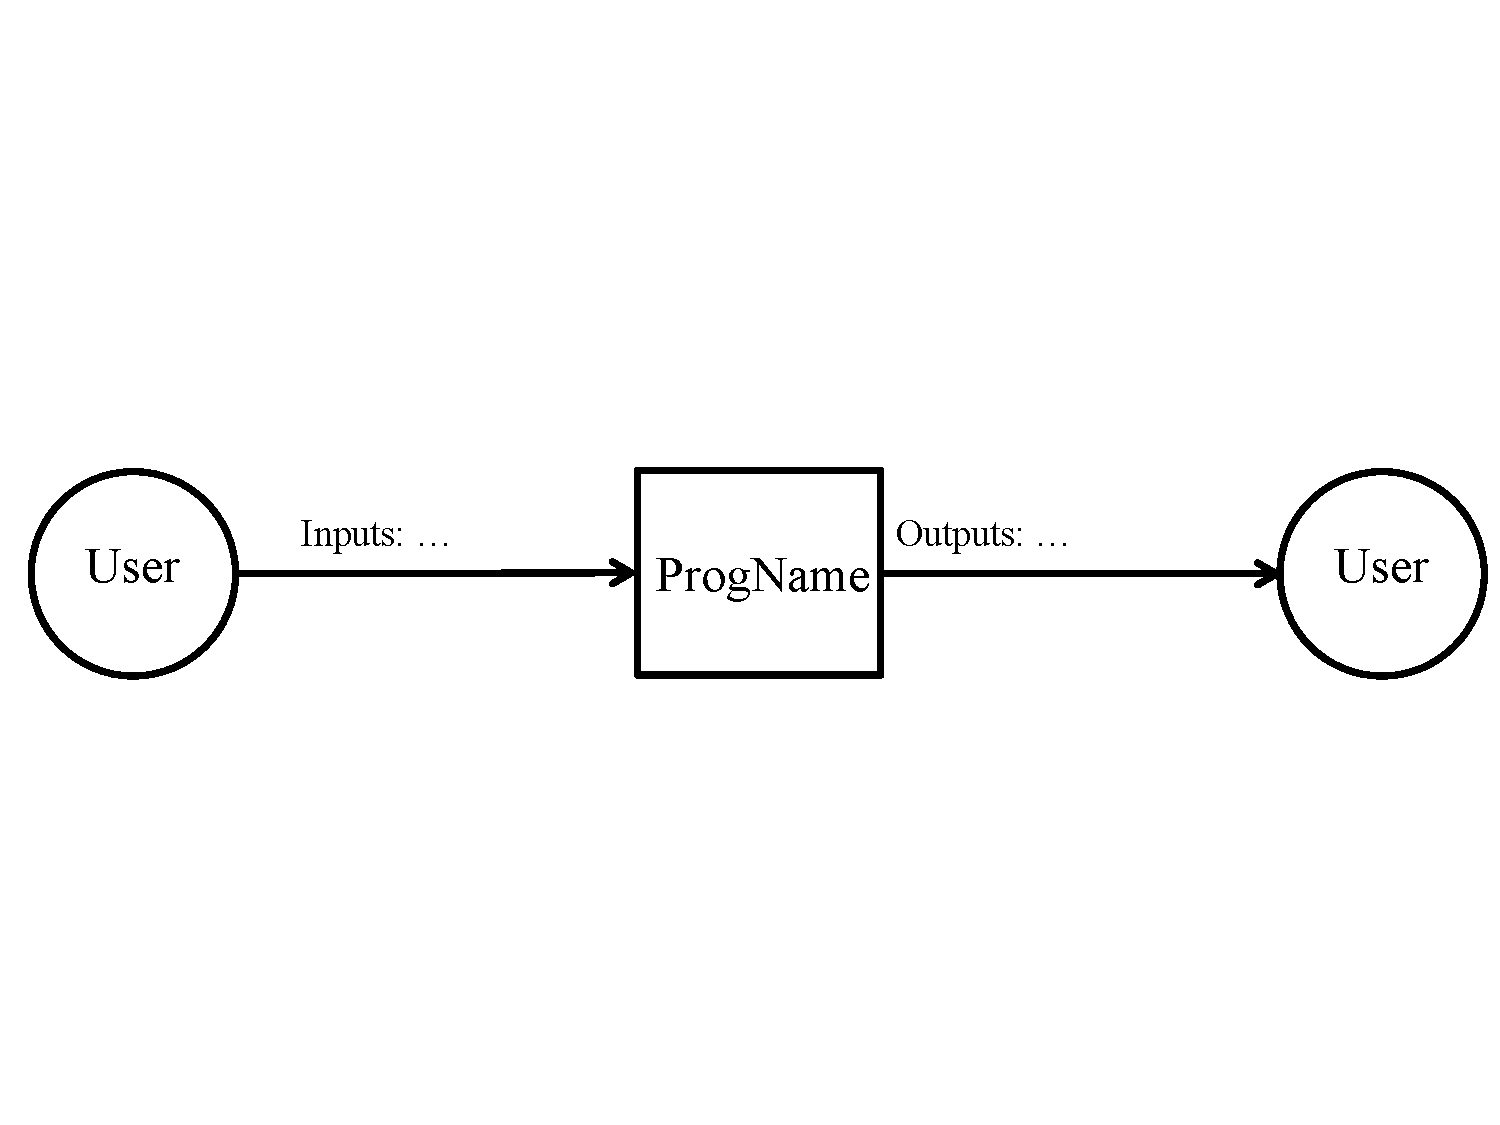
\includegraphics[width=0.6\textwidth]{SystemContextFigure}
			\caption{System Context}
			\label{Fig_SystemContext} 
		\end{center}
	\end{figure}
	
	\plt{For each of the entities in the system context diagram its responsibilities
		should be listed.  Whenever possible the system should check for data quality,
		but for some cases the user will need to assume that responsibility.  The list
		of responsibilities should be about the inputs and outputs only, and they
		should be abstract.  Details should not be presented here.  However, the
		information should not be so abstract as to just say ``inputs'' and
		``outputs''.  A summarizing phrase can be used to characterize the inputs.
		For instance, saying ``material properties'' provides some information, but it
		stays away from the detail of listing every required properties.}
\end{itemize}
	\begin{itemize}
		\item User Responsibilities:
		\begin{itemize}
			\item 
		\end{itemize}
		\item \progname{} Responsibilities:
		\begin{itemize}
			\item Detect data type mismatch, such as a string of characters instead of a
			floating point number
			\item 
		\end{itemize}
	\end{itemize}
	
	\subsection{System Constraints}
	
	\plt{System constraints differ from other type of requirements because they
		limit the developers' options in the system design and they identify how the
		eventual system must fit into the world. This is the only place in the SRS
		where design decisions can be specified.  That is, the quality requirement for
		abstraction is relaxed here.  However, system constraints should only be
		included if they are truly required.}
	
	\subsection{System Scope}
	
	
	\section{Functional Requirements}
	\subsection{The Scope of the Work}
	\subsubsection{The Current Situation}
	N/A
	\subsubsection{The Context of the Work}
	N/A
	\subsubsection{Work Partitioning}
	\begin{center}
    \begin{tabular}{ |c|c|c| } 
     \hline
     \textbf{Event Name} & \textbf{Input and Output} & \textbf{Summary} \\ 
     Creating a Program  & Program Creation \(input\) & Finalizing all program creation inputs from user  \\ 
     Leaving a review on a user's post & Writing a review \(input\) & Commenting and proving a numeric value for program value \\
     Searching for a Program & Program Search \(input\) & Searching and browsing for a specific program or type of program based on search parameters  \\ 
     Sorting search results & Results sorted and displayed \(output\) & Sorting search results in a relevant way that is useful to the user \\ 
     Adding performed sets and reps for exercise & Entering rep and set information \(input\) & Tracking workout information by adding sets and reps performed during exercise \\ 
     Registering an account & Creating a new account \(input\) & This creates a new user and appends it to the database \\ 
     Adding program to profile  & Appending a program to personal profile \(input\) & Users can add programs they find to their profiles to use a later time or immediately \\ 
     Logging into account & Entering account information \(input\) & This authenticates and authorizes the user to access their account  \\ 
     Providing users with suggested programs and workouts & Generating and displaying programs and workouts tailored to individual users \(output\) & Using specific algorithms that find programs that suit the users needs \\ 
     Providing user with statistics & Generating and displaying statistics \(output\) & This will show users statistics they wouldn't otherwise know about. \\ 
     \hline
    \end{tabular}
    \end{center}
	\subsection{The Scope of the Product}
	\subsubsection{Use cases}
	
	\begin{itemize}
		\item View posted workout routine 
		\begin{enumerate}
			\item View other user's fitness progress
			\item Add Personal Workout List
			\item View workout Author
			\item Review workout
		\end{enumerate}
		
		\item Browse Workout routines
		\begin{enumerate}
			\item Filter routines
		\end{enumerate}
		
		\item View Another User's Profile
		\begin{enumerate}
			\item View user's created routines
		\end{enumerate}
		
		\item Create User Profile
		\begin{enumerate}
			\item Setup profile description
			\item Setup attributes
		\end{enumerate}
		
		\item Edit User Profile
		
		\item Start workout routine
		\begin{enumerate}
			\item Track exercises in-progress
			\item Track personal Quantifiers
			\item Update current routine
		\end{enumerate}
		
		
		\item Create workout routine
		\begin{enumerate}
			\item Post workout routine
			\item Categorize routine
			\item Add workout length details
			\item Add exercise 
			\begin{enumerate}
				\item Add Quantifier
				\item Add Workout Descriptions
			\end{enumerate}
		\end{enumerate}
		
		\item Edit Routine
		\item Remove Routine
		\item View Workout List
	\end{itemize}
	
	\subsubsection{Use case Diagram}
	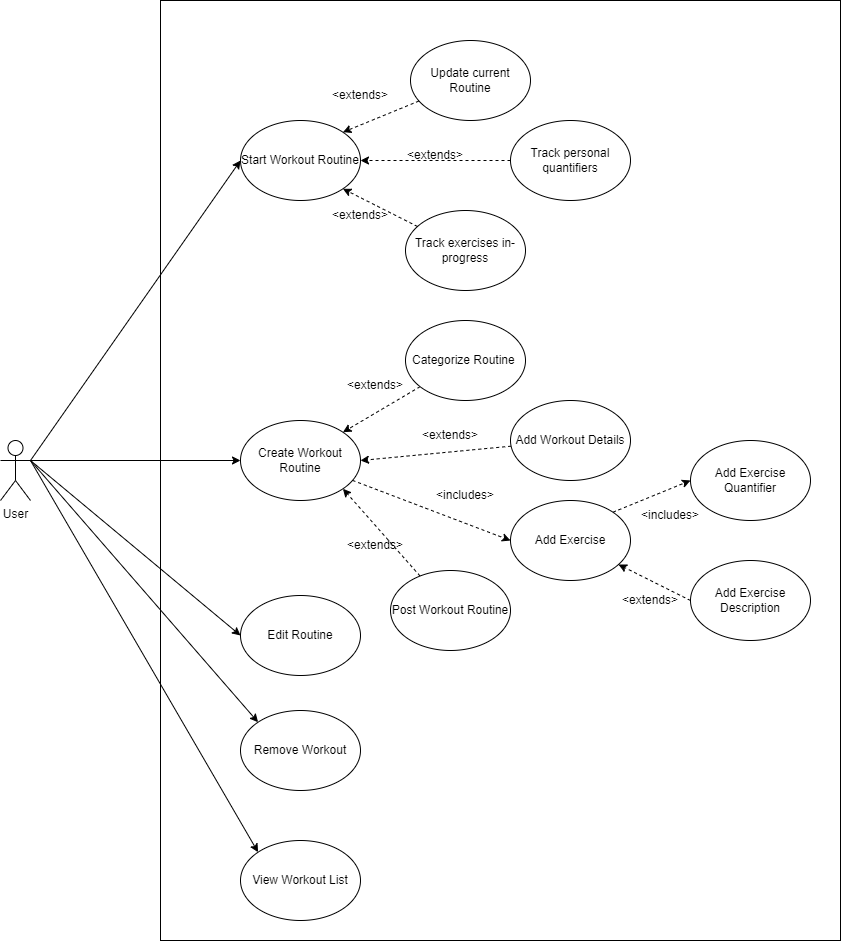
\includegraphics[scale=0.5]{srs_usecase_diagram_routines}
	\newpage
	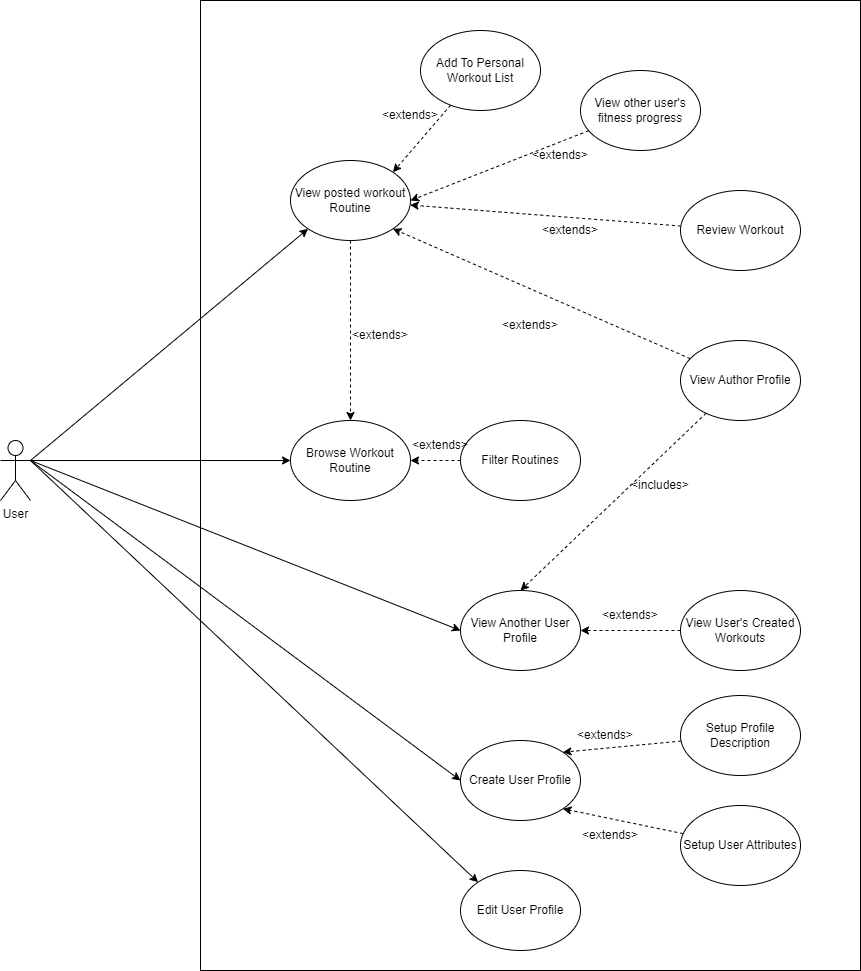
\includegraphics[scale=0.5]{srs_usecase_diagram_profiles}
	
	
	\section{Traceability Matrices and Graphs}
	
	The purpose of the traceability matrices is to provide easy references on what
	has to be additionally modified if a certain component is changed.  Every time a
	component is changed, the items in the column of that component that are marked
	with an ``X'' may have to be modified as well.  Table~\ref{Table:trace} shows
	the
	dependencies of theoretical models, general definitions, data definitions, and
	instance models with each other. Table~\ref{Table:R_trace} shows the
	dependencies of instance models, requirements, and data constraints on each
	other. Table~\ref{Table:A_trace} shows the dependencies of theoretical models,
	general definitions, data definitions, instance models, and likely changes on
	the assumptions.
	
	\plt{You will have to modify these tables for your problem.}
	
	\plt{The traceability matrix is not generally symmetric.  If GD1 uses A1, that
		means that GD1's derivation or presentation requires invocation of A1.  A1
		does not use GD1.  A1 is ``used by'' GD1.}
	
	\plt{The traceability matrix is challenging to maintain manually.  Please do
		your best.  In the future tools (like Drasil) will make this much easier.}
	
	\afterpage{
		\begin{landscape}
			\begin{table}[h!]
				\centering
				\begin{tabular}{|c|c|c|c|c|c|c|c|c|c|c|c|c|c|c|c|c|c|c|c|}
					\hline
					& \aref{A_OnlyThermalEnergy}& \aref{A_hcoeff}& \aref{A_mixed}& \aref{A_tpcm}&
					\aref{A_const_density}& \aref{A_const_C}& \aref{A_Newt_coil}& \aref{A_tcoil}&
					\aref{A_tlcoil}& \aref{A_Newt_pcm}& \aref{A_charge}& \aref{A_InitTemp}&
					\aref{A_OpRangePCM}& \aref{A_OpRange}& \aref{A_htank}& \aref{A_int_heat}&
					\aref{A_vpcm}& \aref{A_PCM_state}& \aref{A_Pressure} \\
					\hline
					\tref{T_COE}        & X& & & & & & & & & & & & & & & & & & \\ \hline
					\tref{T_SHE}        & & & & & & & & & & & & & & & & & & & \\ \hline
					\tref{T_LHE}        & & & & & & & & & & & & & & & & & & & \\ \hline
					\dref{NL}           & & X& & & & & & & & & & & & & & & & & \\ \hline
					\dref{ROCT}         & & & X& X& X& X& & & & & & & & & & & & & \\ \hline
					\ddref{FluxCoil}    & & & & & & & X& X& X& & & & & & & & & & \\ \hline
					\ddref{FluxPCM}     & & & X& X& & & & & & X& & & & & & & & & \\ \hline
					\ddref{D_HOF}       & & & & & & & & & & & & & & & & & & & \\ \hline
					\ddref{D_MF}        & & & & & & & & & & & & & & & & & & & \\ \hline
					\iref{ewat}         & & & & & & & & & & & X& X& & X& X& X& & & X \\ \hline
					\iref{epcm}         & & & & & & & & & & & & X& X& & & X& X& X& \\ \hline
					\iref{I_HWAT}       & & & & & & & & & & & & & & X& & & & & X \\ \hline
					\iref{I_HPCM}       & & & & & & & & & & & & & X& & & & & X & \\ \hline
					\lcref{LC_tpcm}     & & & & X& & & & & & & & & & & & & & & \\ \hline
					\lcref{LC_tcoil}    & & & & & & & & X& & & & & & & & & & & \\ \hline
					\lcref{LC_tlcoil}   & & & & & & & & & X& & & & & & & & & & \\ \hline
					\lcref{LC_charge}   & & & & & & & & & & & X& & & & & & & & \\ \hline
					\lcref{LC_InitTemp} & & & & & & & & & & & & X& & & & & & & \\ \hline
					\lcref{LC_htank}    & & & & & & & & & & & & & & & X& & & & \\
					\hline
				\end{tabular}
				\caption{Traceability Matrix Showing the Connections Between Assumptions and
					Other Items}
				\label{Table:A_trace}
			\end{table}
		\end{landscape}
	}
	
	\begin{table}[h!]
		\centering
		\begin{tabular}{|c|c|c|c|c|c|c|c|c|c|c|c|c|c|c|c|c|c|c|c|c|c|c|c|}
			\hline        
			& \tref{T_COE}& \tref{T_SHE}& \tref{T_LHE}& \dref{NL}& \dref{ROCT} &
			\ddref{FluxCoil}& \ddref{FluxPCM} & \ddref{D_HOF}& \ddref{D_MF}& \iref{ewat}&
			\iref{epcm}& \iref{I_HWAT}& \iref{I_HPCM} \\
			\hline
			\tref{T_COE}     & & & & & & & & & & & & & \\ \hline
			\tref{T_SHE}     & & & X& & & & & & & & & & \\ \hline
			\tref{T_LHE}     & & & & & & & & & & & & & \\ \hline
			\dref{NL}        & & & & & & & & & & & & & \\ \hline
			\dref{ROCT}      & X& & & & & & & & & & & & \\ \hline
			\ddref{FluxCoil} & & & & X& & & & & & & & & \\ \hline
			\ddref{FluxPCM}  & & & & X& & & & & & & & & \\ \hline
			\ddref{D_HOF}    & & & & & & & & & & & & & \\ \hline
			\ddref{D_MF}     & & & & & & & & X& & & & & \\ \hline
			\iref{ewat}      & & & & & X& X& X& & & & X& & \\ \hline
			\iref{epcm}      & & & & & X& & X& & X& X& & & X \\ \hline
			\iref{I_HWAT}    & & X& & & & & & & & & & & \\ \hline
			\iref{I_HPCM}    & & X& X& & & & X& X& X& & X& & \\
			\hline
		\end{tabular}
		\caption{Traceability Matrix Showing the Connections Between Items of Different
			Sections}
		\label{Table:trace}
	\end{table}
	
	\begin{table}[h!]
		\centering
		\begin{tabular}{|c|c|c|c|c|c|c|c|}
			\hline
			& \iref{ewat}& \iref{epcm}& \iref{I_HWAT}& \iref{I_HPCM}&
			\ref{sec_DataConstraints}& \rref{R_RawInputs}& \rref{R_MassInputs} \\
			\hline
			\iref{ewat}            & & X& & & & X& X \\ \hline
			\iref{epcm}            & X& & & X& & X& X \\ \hline
			\iref{I_HWAT}          & & & & & & X& X \\ \hline
			\iref{I_HPCM}          & & X& & & & X& X \\ \hline
			\rref{R_RawInputs}     & & & & & & & \\ \hline
			\rref{R_MassInputs}    & & & & & & X& \\ \hline
			\rref{R_CheckInputs}   & & & & & X& & \\ \hline
			\rref{R_OutputInputs}  & X& X& & & & X& X \\ \hline
			\rref{R_TempWater}     & X& & & & & & \\ \hline 
			\rref{R_TempPCM}       & & X& & & & & \\ \hline
			\rref{R_EnergyWater}   & & & X& & & & \\ \hline
			\rref{R_EnergyPCM}     & & & & X& & & \\ \hline
			\rref{R_VerifyOutput}  & & & X& X& & & \\ \hline
			\rref{R_timeMeltBegin} & & X& & & & & \\ \hline
			\rref{R_timeMeltEnd}   & & X& & & & & \\ 
			\hline
		\end{tabular}
		\caption{Traceability Matrix Showing the Connections Between Requirements and
			Instance Models}
		\label{Table:R_trace}
	\end{table}
	
	The purpose of the traceability graphs is also to provide easy references on
	what has to be additionally modified if a certain component is changed.  The
	arrows in the graphs represent dependencies. The component at the tail of an
	arrow is depended on by the component at the head of that arrow. Therefore, if a
	component is changed, the components that it points to should also be
	changed. Figure~\ref{Fig_ATrace} shows the dependencies of theoretical models,
	general definitions, data definitions, instance models, likely changes, and
	assumptions on each other. Figure~\ref{Fig_RTrace} shows the dependencies of
	instance models, requirements, and data constraints on each other.
	
	\section{Project Issues}
	\subsection{Open Issues}
	\subsection{Off the Shelf Solutions}
	\subsection{New Problems}
	\subsection{Tasks}
	\subsection{Migration to the New Product}
	\subsection{Risks}
	\subsection{Costs}
	\subsection{User Documentation and Training}
	\subsection{Waiting Room}
	\subsection{Ideas for Solutions}
	
	
	
	\section{Reference Material}
	
	This section records information for easy reference.
	
	
	\subsection{Abbreviations and Acronyms}
	
	\renewcommand{\arraystretch}{1.2}
	\begin{tabular}{l l} 
		\toprule		
		\textbf{symbol} & \textbf{description}\\
		\midrule 
		A & Assumption\\
		DD & Data Definition\\
		GD & General Definition\\
		GS & Goal Statement\\
		IM & Instance Model\\
		LC & Likely Change\\
		PS & Physical System Description\\
		R & Requirement\\
		SRS & Software Requirements Specification\\
		\progname{} & \plt{put an expanded version of your program name here (as
			appropriate)}\\
		T & Theoretical Model\\
		\bottomrule
	\end{tabular}\\
	
	\plt{Add any other abbreviations or acronyms that you add}
	
	% \begin{figure}[h!]
		% 	\begin{center}
			% 		%\rotatebox{-90}
			% 		{
				% 			\includegraphics[width=\textwidth]{ATrace.png}
				% 		}
			% 		\caption{\label{Fig_ATrace} Traceability Matrix Showing the Connections
				%Between Items of Different Sections}
			% 	\end{center}
		% \end{figure}
	
	
	% \begin{figure}[h!]
		% 	\begin{center}
			% 		%\rotatebox{-90}
			% 		{
				% 			\includegraphics[width=0.7\textwidth]{RTrace.png}
				% 		}
			% 		\caption{\label{Fig_RTrace} Traceability Matrix Showing the Connections
				%Between Requirements, Instance Models, and Data Constraints}
			% 	\end{center}
		% \end{figure}
	
	\newpage
	
	\bibliographystyle {plainnat}
	\bibliography {../../refs/References}
	
	\newpage
	
	\noindent \plt{The following is not part of the template, just some things to
		consider
		when filing in the template.}
	
	\noindent \plt{Grammar, flow and \LaTeX advice:
		\begin{itemize}
			\item For Mac users \texttt{*.DS\_Store} should be in \texttt{.gitignore}
			\item \LaTeX{} and formatting rules
			\begin{itemize}
				\item Variables are italic, everything else not, includes subscripts (link to
				document)
				\begin{itemize}
					\item \href{https://physics.nist.gov/cuu/pdf/typefaces.pdf}{Conventions}
					\item Watch out for implied multiplication
				\end{itemize}
				\item Use BibTeX
				\item Use cross-referencing
			\end{itemize}
			\item Grammar and writing rules
			\begin{itemize}
				\item Acronyms expanded on first usage (not just in table of acronyms)
				\item ``In order to'' should be ``to''
			\end{itemize}
	\end{itemize}}
	
	\noindent \plt{Advice on using the template:
		\begin{itemize}
			\item Difference between physical and software constraints
			\item Properties of a correct solution means \emph{additional} properties, not
			a restating of the requirements (may be ``not applicable'' for your problem).
			If you have a table of output constraints, then these are properties of a
			correct solution.
			\item Assumptions have to be invoked somewhere
			\item ``Referenced by'' implies that there is an explicit reference
			\item Think of traceability matrix, list of assumption invocations and list of
			reference by fields as automatically generatable
			\item If you say the format of the output (plot, table etc), then your
			requirement could be more abstract
		\end{itemize}
	}
	
	\newpage{}
	\section*{Appendix --- Reflection}
	
	The information in this section will be used to evaluate the team members on the
	graduate attribute of Lifelong Learning.  Please answer the following questions:
	
	\begin{enumerate}
		\item What knowledge and skills will the team collectively need to acquire to
		successfully complete this capstone project?  Examples of possible knowledge
		to acquire include domain specific knowledge from the domain of your
		application, or software engineering knowledge, mechatronics knowledge or
		computer science knowledge.  Skills may be related to technology, or writing,
		or presentation, or team management, etc.  You should look to identify at
		least one item for each team member.
		\item For each of the knowledge areas and skills identified in the previous
		question, what are at least two approaches to acquiring the knowledge or
		mastering the skill?  Of the identified approaches, which will each team
		member pursue, and why did they make this choice?
	\end{enumerate}
	
\end{document}
